\section{Optimization System}
\label{optimization}
In this section I discuss optimization of coordination and describe the optimization method I later use to extend DOGS into address the coordination issues I introduced in section \ref{dogs}.

\subsection{Coordination}
\label{coordination}
Coordination along an arterial is fundamental in signal optimization. The ideal situation for road users is the \textit{green wave}, where upon arrival to the next intersection there will always be a green light.

Contemporary car engines consume less fuel in general when they are allowed to run at a constant RPM level so the travel experience as well as emmission levels are improved under coordination.

There are also security aspects which indicate that coordination and green waves are desirable since the human eye has difficulty in observing acceleration and deceleration.

In one-way coordination a signal controller emits a platoon of vehicles over a period of time, say from $t_1$ to $t_2$, where $T_g = t_2 - t_1$ ie. the green time is indicative of the number of vehicles that need to pass. To avoid stopping these vehicles at the next signal the same amount of green time, $T_g$ must be given to the approaching platoon only \textit{offset} in time by $\Delta f$ to represent the travel time of the platoon from one signal to the next. 

In fact, due to \textit{platoon dispersion}, which depend mainly on the intersignal distance and speeds, more than $T_g$ green time must be allotted to the stage of the downstream signal. It is also due to platoon dispersion that coordination is only relevant for signals which are relatively close. Practical experience from DRD indicate that the distance should not exceed 800-900 m. 

In perfect two-way coordination between two intersections the leading vehicles in platoons of traffic in either direction must experience that the next signal switch to green before they reach the area in which they decide to brake for red.

In a common cycle-time based system \cite{coord} gives us:

$$o = n \cdot \frac{C}{2}$$

Where $o$ is the travel time between the intersections, which is assumed to be the same in both directions, $C$ is the cycle time and $n$ is an integer.

The travel time is calculated as $o = L / v$ where $L$ is the distance and $v$ is the speed by which road users travel between the intersections. By insertion we get:

$$C = 2 \cdot \frac{L}{n \cdot v}$$

This equation is quite constrained, however. For cycle time we require that it lies within a span of about 60 til 120 seconds based on recommendations from DRD. If the cycle time is less, stage lengths become too short to reach past the queue startup delay (about 4 vehicles), if more the minor roads experience long delays and pedestrians and bicyclists may start to cross the road before the signal turns green.

In addition green waves usually span over more than two intersections which may have different distances and average speeds between them, all this making it hard or impossible to find an integer $n$ satisfying the constraints. Thus green waves are most easily established in one, main direction. It is possible to affect the average speeds between intersections by changing the allowed speed-signs. If this is not sufficient one might accept that the green wave is not perfect by, for instance, prioritizing one direction over the other.

Priority can be given entirely to one direction or distributed by some weight, for instance based on the ratio of traffic in each direction. An obvious choice for the first option would be for an arterial with traffic between some suburbs and a major city. In the morning full priority should be given in the direction towards the city when people go to work and opposite in the afternoon. A third alternative is to provide a perfect progression band in one direction for a some ratio of time, corresponding to the ratios of traffic in either direction.
For ringroad 3, which was simulated in this project, there is no profound direction bias in the morning or afternoon traffic (see section \ref{data}) and a solution which weighs the green wave quality according to direction ratio is preferred. 

The distance between one signal head (intersection) and the next can be extracted from the Vissim network file in both directions and is static. The signal heads for both directions of the arterial are marked using a naming convention similar to the one mentioned in Section \ref{routefractions} only less information is required since the relation of the head to its signal controller can be deduced directly from the network file. Further details on this process can be read in Section \ref{signal_details}.

For travel times (which is a key component in finding a proper offset) it is possible to rely on the speed limitations / free flow speeds for offset calculation, however under congestion speeds will decrease causing the travel times to increase. A better solution is to continuously inspect the smoothened travel times which are inserted for each stretch. 

\subsection*{Why are we using common cycle schemes?}
\label{phase_based}
In this section I highlight the restrictions imposed when introducing two-way coordination between common cycle time signal controllers. Are there no alternatives, which are less strict and why aren't they used in Denmark?

With a common cycle time comes fixed signal plans that give us full insight into the operation of the each signal controller. We can see exactly which signal groups ie. heads are green, red, yellow and amber at any given second. Furthermore, as presented above, there exist expressions for the offset and cycle time which causes coordination. 

Although traffic actuated green time extension schemes exist to make fine adjustsmens, such as the ones used for bus priority, it is always necessary to take the seconds from some other stage due to the common cycle time requirement. Likewise with stage skipping, you must always "spend" $C$ cycle seconds - and may never spend more - before restarting the signal plan.

These restrictions makes it difficult for a computer system to obtain optimum performance for the signal controllers and the observed / predicted traffic.

In addition, for large networks the enforcement of a common cycle time is inappropriate. Consider a network which is so large that two disjoint arterials exist (such as the case of ringroad 3 - Herlev and Glostrup). In this case it is unlikely that a common cycle time will allow green waves to exist for both arterials eg. when the intersections of one arterial are more tightly spaced than in the other. Even though the arterials cannot be considered as a single arterial, they are not completely disjoint and will affect each other, if relatively close.

Stage based signals is an alternative to fixed signal plans where stages are queued for future execution along with a green time. There is no fixed order of the stages and no fixed green time. This gives great flexibility for the computer system, however the problem is the plans cannot be written down in advance in terms of $C$ for human inspection and control. Instead they must be defined dynamically on the basis of a set of signal rules, which are implemented and respected by the computer system while adapting to the measured traffic conditions. 

Here is a subset of rules such a system should implement:

\begin{description}
\item[Coordination]
Whenever the arterial stage for a signal is active from $t_1$ to $t_2$ the arterial stage of the downstream signal should be active from $t_1 + o$ to $t_2 + o$ where $tt$ is the best estimate of travel time from signal 1 to signal 2.
\item[Priority for the arterial]
The green times for all stages in the direction of the arterial must match the load on the arterial, respecting other rules.
\item[Fairness to minor roads]
The queues for minor roads cannot exceed a predefined length nor must a vehicle wait more than a certain amount of time at any intersection to pass.
\end{description}

These rules - given proper parameters - are precise enough to be implemented in a computer program. The setting of parameters (for instance maximum queue length for minor roads) is a difficult subject, which could require many training hours for end-users. This was my impression about the Utopia/Spot system which the municipality of Copenhagen (Vej \& Park) had implemented for Centrum Forbindelsen - its was difficult for them to decide on which adjustsments should be made, when the system acted up. 
However, many parameters can - and should - be set automatically by repeated simulation with trial-and-error or they are either easy enough to understand that rules of thumb and area specific insight is enough to make proper choices.

I believe stage based signals and more centralized computer control of arterials could be accepted and achieved if systems were more available and open as proposed above. The introduction of stage based signals would be a major break with tradition in Denmark - and probably also in many other countries. Some systems exist, which use stage-based programs including RHODES \cite{rhodes} and UTOPIA/SPOT \cite{utopia_spot} mentioned previously.

Breaking tradition is always hard; this combined with the complexity of such a system has compelled me to remain in the common cycle time world in this project. But as will be seen in the following sections, there are many ways to improve arterial signal performance in spite of the the restrictions of $C$.

\subsection{Manipulating speed}
The first option, which is implemented in the search procedure (see section \ref{siman}), is to improve coordination by affecting the speeds of road users. This is done by adjusting speed signs since most motorists will obey these. The travel time between intersections, which largely determines the offset, could then be increased or decreased by changing the speed signs. 

In Figure \ref{fig:change_speed} we can see how this works. In the \textit{before} situation, platoons from intersection $i+1$ arrive too late and some experience red light. In the \textit{after} situation, the platoon is allowed to go faster and arrive entirely during the green time of intersection $i$.

\begin{figure}[htbp]
\centering
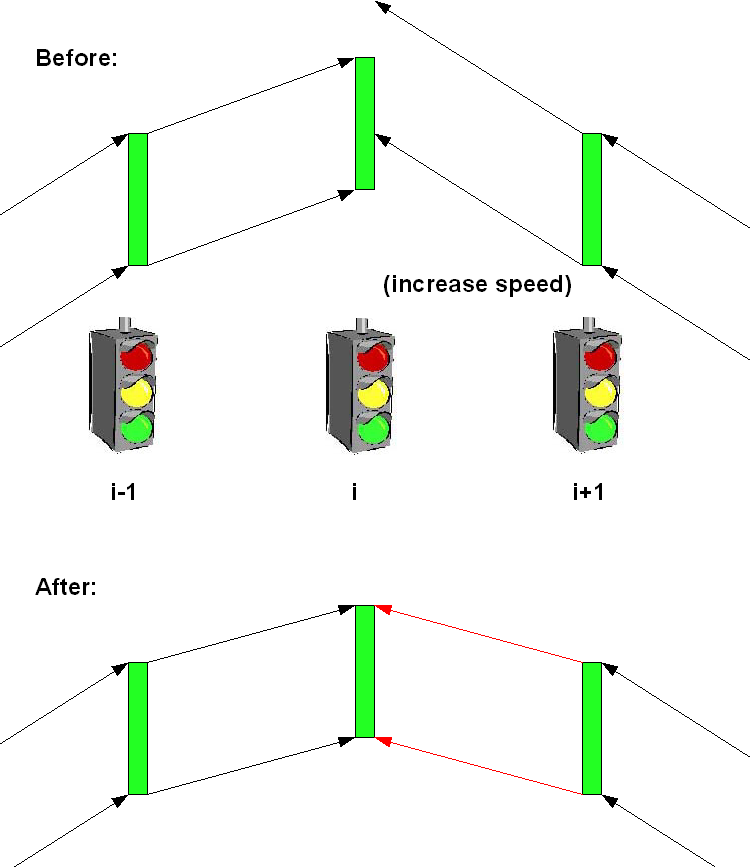
\includegraphics[scale=0.3]{change_speed.png}
\caption{Changing speeds to obtain better coordination}
\label{fig:change_speed}
\end{figure}

Some considerations should be made in this respect. For instance we must ensure that the speeds do not divert too much from the norm of the relevant type of road. In addition the number of speed changes, which a motorist travelling throughout the arterial experience, must be minimized. And if speed changes do occur, it is a good idea to keep them small so that the speeds don't go from 50 to 70 from one stretch of road to the next.

From a security perspective it might seem risky to not persist a common speed level through the artery. But considering that a change of speed might improve the quality of the coordination, this problem is negated. This also applies to the additional acceleration and deceleration since, if a green wave does not exist the vehicles must be stopped altogether at the red light causing even more acceleration.

The current infrastructure on O3 does not offer this fine-grained level of adjustment but electronic speed signs are common practice nowadays and is, for instance, used on the almost-parallel motorring 3 to smoothen out queues.

\subsection{Adjusting offsets}
The individual signal offset is the traditional parameter for adjustment. The formulas presented earlier (section \ref{coordination}) can be used to establish one-way coordination, under the restrictions described, but two-way coordination is not solved so easily.

Traditional offline optimization systems such as TRANSYT often employs a black-box simulator for fitness evaluation. However for offsets we can do without such overhead since we know exactly what we are looking for.

Basically the purpose of offsets is to properly align adjacent intersections in time such that a platoon emitted during the green time of intersection 1 is met by a green light at the adjacent intersection 2. A good estimate of the propagation time of the platoon is the travel time $tt_{1,2} = d / v$ where $v$ is the average speed and $d$ is the distance between the intersections and the green time displacement, $\Delta f_{i,j}$, should match $tt$ for all adjacent intersections $i$ and $j$.

\begin{figure}[htbp]
\centering
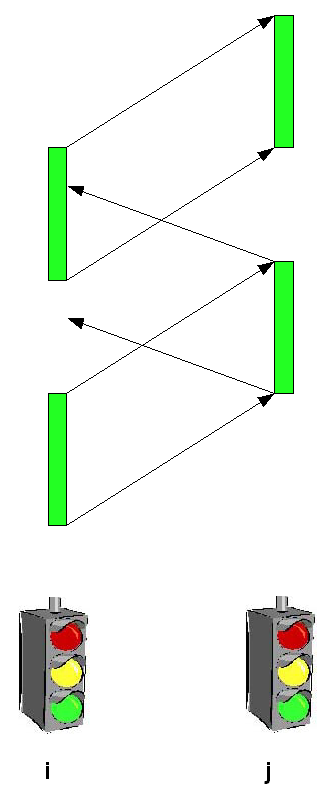
\includegraphics[scale=0.4]{change_offset.png}
\caption{Changing offsets to obtain better coordination}
\label{fig:change_offset}
\end{figure}

We can change both the travel time, by changing speed signs, and also the green time displacement by adjusting offsets. The consequences of changing an offsets can be difficult to foresee, consider the example in Figure \ref{fig:change_offset}. From intersection $j$ to $i$ the platoon will arrive too early. We can increase the offset (delay the green start) of $j$ but then we just reverse the situation. During all this, we must expect that there are also signal controllers $i-1$ and $j+1$ to the left and right resp. of $i$ and $j$, which must be in coordination with $i$ and $j$.

Metaheuristic search procedures are designed to cope with situations such as these where the immediate effects of a change cannot be foretold.

\subsection{Direction bias}
In section \ref{data} we looked at the detector data and traffic counts, which are used to fit the simulation. We saw, among other things, that there northgoing traffic is higher than southgoing. The optimization routine can be coherced into favoring one direction over the other - or be completely fair - by punishing deviations from a certain bias indicator.

To calculate the bias under current offsets we sum, in each direction of the artery, the deviations of the green time displacement to the expected travel time. The bias is thus the ratio of these sums and can be compared to the desired bias. The punishment for choosing settings, which result in deviation from the desired bias, is a factor which grows exponentially with deviations in either direction.

By using such a weight the effect is that eg. perfect coordination in one direction - on the cost of coordination in the opposite direction - will be heavily punished under neutral bias (identity). This method can also be used to establish highly direction specific coordinations when the bias approaches zero or infinity.

\subsection{Closely distanced intersections}
When the distance from an intersection to the upstream intersection is short (eg. $\leq 200 m$) coordination between the two intersections should receive special attention for two reasons:

\begin{itemize}
\item Since they are closely distanced queues cannot be very long before reaching back to the downstream intersection
\item Travel time between the intersections is more predictable since the natural variations in speeds do not have much time to work in forming platoons unlike for longer stretches of intermediate road, where the travel time spread is higher
\end{itemize}

To favorize good coordination between closely distanced intersection I have chosen to use weights.  I have opted to not statically classify what is close and what is not but rather rank the distances of all coordinations between adjacent intersections and set the weight of imperfections accordingly. The effect is that flaws in coordinations between close intersections adds more to the total solution value than for the same flaws at widely spaced intersections and thus the minimization problem solver is guided toward favorizing coordination between close intersections.

\subsection{Metaheuristic search}
DRD has traditionally used TRANSYT to obtain coordination. TRANSYT employs a genetic algorithm to finds its solutions but often it is necessary to manually adjust the offsets in order to obtain a good two-way coordination or to give preference to some direction. 

This manual process involves creating good two-way green waves by compromise, which could be either some sacrifice in the quality of the green waves. 

In this project the green wave concept has been formalized so that it is possible to evaluate a proposal for offsets. This opens up for the application of a metaheuristic search procedure.

In this cycle-based approach the variable to be optimized is, of course, the offset for each signal controller. The signal controllers themselves operate under cyclic plans which are shifted in time according to the chosen offset. In addition all above suggestions for improved coordination are implemented.

\subsubsection*{Evaluation of solutions}
\label{eval_coord}
For non-trivial arteries of size $n \geq 2$ intersections there are $n$ offsets to select and $m = 2 \cdot n - 2$ coordinations\footnote{Since each signal controller has an outgoing coordination in each direction except at the ends, which have only one} and hence $m$ speeds to choose, assuming speeds and distances are \textit{not} symmetric in the coordination from signal controller $i$ to $j$ and $j$ to $i$.
The selection of offsets and speeds is a minimization problem where the fitness value indicates the quality of a coordination:

$$ \min \sum_{\forall i,j} f(o_i,o_j,s_{ij})$$

Where $i$ and $j$ are signal controllers, $o$ is the offset vector, $s$ contains speeds for each coordination and $f$ is the fitness function. The common cycle time is fundamental in the evaluation, but is not an optimization variable in this context and is thus not shown here.

I previously hinted at various methods of evaluating the fitness of solutions to offsets (and speeds). The most general approach is by using a simulator, however we cannot use Vissim for this purpose, as mentioned in section \ref{simulation}, due to the fact that Vissim runs - at best - at 10-50 times realtime speed in the network used in this project on contemporary machines. Using metaheuristics we need to evaluate several hundreds of solutions - and preferably more - per second and thus Vissim is far too slow for this purpose.

Since we only solve a subproblem of signal setting optimization, \textit{coordination}, we can exploit the nature of coordination and below are three suggestions, listed in order of increasing complexity, I have found to evaluate solutions to coordination.

\begin{description}
\item[Green time displacement]
The simplest - but most constrained - evaluation criterion. As explained in Figure \ref{fig:green_time_displacement}, section \ref{dogs_offset}, the start of greens are aligned by changing offsets so that the difference between travel time (given the average travel speed) and green time displacement is minimized for all coordinations:

$$|\Delta f - traveltime|$$

\item[Green time displacement considering length of green times]
In the above evaluation method only green starts are considered. If the green durations of the signal controllers being coordinated are not equally long it is possible to introduce some flexibility, as can be seen in Figure \ref{fig:green_time_displacement_flex}.

\begin{figure}[htbp]
\centering
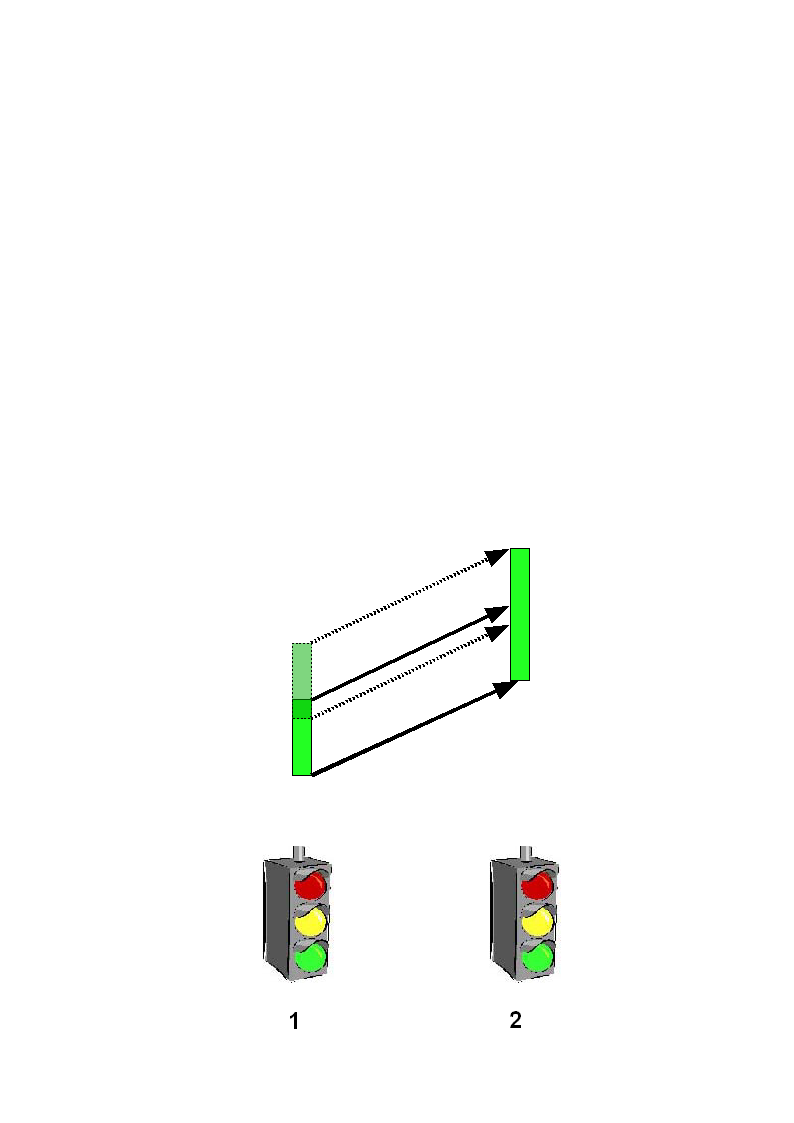
\includegraphics[scale=0.4]{green_time_displacement_flex.png}
\caption{Flexibility in green time displacement considering downstream green duration}
\label{fig:green_time_displacement_flex}
\end{figure}

Since the duration of the downstream green time is longer, the green start (offset) of the first signal controller can be chosen more freely without sacrificing coordination. This increases the count of good solutions, since now several solutions yield the same solution value due to the addded flexibility and allows the solver to find better solutions.

\item[Horizon evaluation]
The final suggestion is an extension of the previous scheme. It is suited for evaluating coordination for common cycle time, fixed signal plan controllers as well as stage based signal controllers.

For evaluation of a \textit{coordination} from signal controller $i$ to $j$ in the context of a time horizon $H = h_{min} .. h_{max}$ we examine each \textit{green band}, which is emitted from $i$. Here a band is understood as an integer set of seconds in the horizon from the green start to green end of a signal controller (see eg. Figure \ref{fig:green_time_displacement_flex}).

Given the distance and chosen speed in the coordination we can shift the band emitted from signal controller $i$, called $b1$, by the travel time, and, by comparing the resulting band to the equivalent band of the downstream controller $j$, called $b2$, count how many seconds worth of green band, which is not being "let through". Band $b1$ may be cut in several ways, if it is not fully compatible with $b2$ ie. the downstream controller does not provide a green light for all traffic from the first controller:

\begin{itemize}
\item There is no overlap. This is the worst situation that happens when all traffic from the first signal controller will be met by a red light at the downstream controller. The fitness is the size of $b1$.
\item When the beginning of the $b1$ lies before $b2$ the green start of the first controller was too early or the downstream controller started its green too late. This will result in the stopping of the head vehicles from $i$ and the fitness is the size of $b1 \ b2$.
\item Similar to the previous case but $b1$ extends beyond $b2$. Here the tail of vehicles from $i$ is cut off and the fitness is the size of $b2 \ b1$.
\item When $|b1|>|b2|$ there is a chance that both the head and tail of vehicles from the first signal controller are cut since the downstream controller cannot offer enough green time to match that of the previous controller. In this case $b1 \ b2$ will result in two discontinued sequences of seconds in the horizon and the sum of the sizes of the sets constitute the fitness value.
\end{itemize}

This evaluation method is generic since the only requirement is the green bands in the horizon. This information can be extracted from all types of signal controllers, including stage-based controllers with memory of past stages. Pretimed signal controllers does not need memory of past stages to supply information on green times and thus the overhead of this evaluation scheme is not necessary. I believe, however, that this option might be of interest in future works and have left it here for completeness.

\end{description}

In these evaluation methods no attempt is made to address preexisting queues before the arrival of platoons from the downstream intersections. The dynamic nature (length) of these residual queues first mentioned in section \ref{dogs_offset} is not easily handled in a common cycle time signal setting scheme. It is possible to incorporate a buffer for residual queue clearance by reducing the travel time used in the calculations so that it is shorter than the actual travel time. However the problem of finding a \textit{sweet spot} that does not waste green time while clearing queues was beyond the scope of this report.

During testing it was found that the simplest evaluation option, to regard only green time displacements, gave the best results on average and this was chosen as the primary evaluation mechanism in the offset optimization routine. I believe that the reduction in search space and complexity has increased the number of solutions tested per second to a level that the higher freedoms of the latter two solutions did not give an advantage over the simplest evaluation method. Unfortunately I did not have time to properly test this hypothesis.

\subsection{Simulated Annealing}
\label{siman}
In this section I describe the metaheuristic search routine, which was chosen: Simulated Annealing (SA). 
SA is a \textit{hill-climber} with the ability to escape from local optima ie. jump to another hill-top. It builds on ideas of the \textit{annealing} from the metal industry where metals are heated and slowly cooled down to allow the molecules to arrange themselves so that the metal is as strong as possible.

This can be transferred to computer-aided optimization as taking a completely random (ie. "smeltered" solution) and slowly cool it (inspecting neighbor solutions) to find a good solution. Thus SA performs a randomized, converging search in the entire search space (for offsets that is each combination of $N \bmod C$ over the intersections) looking for the possible best set of offsets without getting stuck with the \textit{first-and-best} solution it encounters.

The initial solution is chosen so that all offsets are zero\footnote{Alternatives are, for each controller, a random offset within the common cycle time (by some distribution eg. uniform) or some pre-existing offsets eg. generated by TRANSYT}. SA then works its way toward a better solution by examining neighbor solutions to the current one. A neighbor solution is found by incrementing or decrementing a single offset in the current solution or changing the allowed speed between the intersections by 5$km/h$.

The solutions to offsets are evaluated and compared in the context of the network and, if a neighbor is found to be better than the best solution found so far, it is adopted as the new \textit{encumbent}. If the neighbor was not better it should be thrown away, but here SA avoids being caught in a local optima by \textit{with some probability}, related to the entropy difference of the current and neighbor solutions, keeping the neighbor solution regardless and work on from there. This characteristics of this probability function - which decreases as the search progress  - is chosen manually and so is subject to tuning.

Generally metaheuristics give no guarantee that an optimum solution will be found, but with proper tuning and fast data structures - so that at least a couple of hundred solutions can be tested per second - it is my experience that they will yield good solutions. The strengths of metaheuristics are that they can easily support any kind of constraint, take advantage of the structure of the problem and the running time is bounded only by the time available.

In this project I have developed data structures, which are fast enough to generate the necessary iterations per second and can be used in various metaheuristic search schemes, not just simulated annealing.

In my experience the keys to speed in metaheuristic search are \textit{delta-evaluation} and to avoid \textit{object instantiation}.

\subsubsection{Delta-evaluation}
To evaluate a solution for offsets for sequentially adjacent signal controllers $sc_1$ to $sc_n$ we evaluate, in accordance to description in section \ref{eval_coord}, each coordination $(sc_1,sc_2)$, $(sc_2,sc_1)$\footnote{Coordinations between adjacent signal controllers need not be symmetrical. For instance there might be a longer way in one direction that the other or, more likely, different \textit{speeds} might be allowed} and so forth. This gives us a value for each coordination and we then perform some kind of aggregation in order to obtain a single figure, the solution value, which is augmented using the weighting methods described earlier.

Every time a neighbor solution is generated we normally immediately want to evaluate it as well. This can be done by going through the routine described above, but we can also use delta-evaluation to speed up the evaluation, if we have information on the structure of the problem.

A change in the offset of signal controller $sc_i$ will affect the coordinations between $sc_{i-1}$ and $sc_{i}$ and also between $sc_{i}$ and $sc_{i+1}$. Since we didn't change the offset $sc_{i-1}$ or $sc_{i+1}$ or any other offset, all coordinations but those mentioned will remain just as good - or bad - as before the offset change for $sc_i$. This is illustrated in Figure \ref{fig:delta_eval}.

\begin{figure}[htbp]
\centering
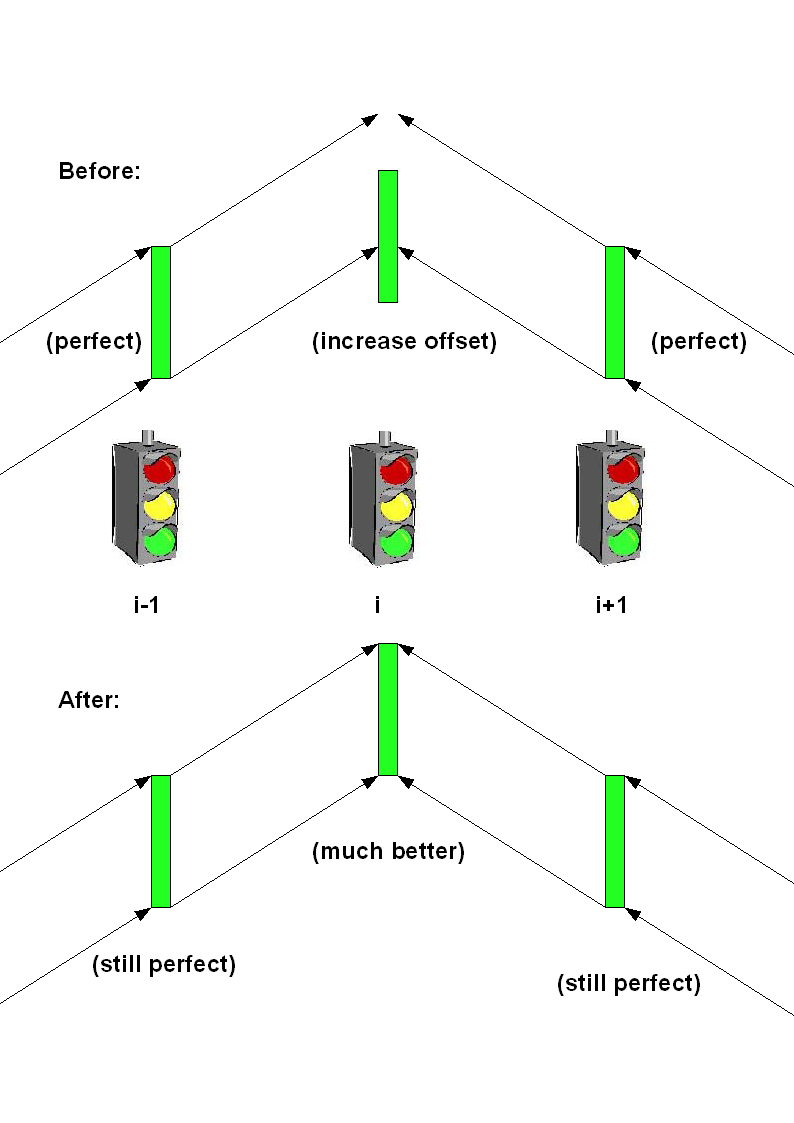
\includegraphics[scale=0.3]{delta_eval.png}
\caption{Local nature of coordinations. This illustrates the quality of coordinations between three signal controllers before and after changing the offset of the middle controller. Notice that the coordinations between the outer controllers and $sc_{i-2}$ and $sc_{i+2}$ remain the same.}
\label{fig:delta_eval}
\end{figure}

So, rather than evaluating every coordination again we may safely assume that only coordinations $(sc_{i-1},sc_{i})$, $(sc_{i-1},sc_{i})$ and $(sc_{i},sc_{i+1})$, $(sc_{i+1},sc_{i})$ need to be reevaluated. 

We now need only to evaluate at most four coordinations\footnote{Changing offsets for controllers in the ends of the arterial will only change the value of two coordinations.} to obtain the neighbor solution value. In total there are $m = 2\cdot (n-1)$ coordinations to evaluate and thus we exchange a linearly growing evaluation time (in the number of signal controllers) for a constant one and rough tests have shown that, even for small networks, the savings in CPU time per iteration are in excess of a factor two, in spite of the extra overhead due to bookkeeping.

\subsubsection{Neighbor solutions}
In previous studies of metaheuristics, where the object oriented programming model was completely adopted, it was found that the overhead of object instantiation, whenever a neighbor solution was generated, would result in tremendous consumption of CPU time. 

Instead I have minimized the need for copying information from a solution to its neighbor by introducing the dual methods \verb|change| and \verb|undo_changes|. The purpose of these methods is to allow a solution to temporarily take the form of its neighbor and switch back to its former self, if requested. 
When the metaheuristic runs it will constantly ask for neighbor solutions but throw away most of them. This approach avoids much copying of solution attributes and at the same time the details of the switching of identify are relayed to the solution object.

\subsubsection{Bookkeeping outline}
The \verb|change| and \verb|undo_changes| methods are closely integrated with delta-evaluation. The initial solution obviously cannot be delta-evaluated so, during full evaluation, the \textit{contribution} from each coordination is noted. 

When \verb|change| is called a signal controller whose offset to change is chosen as well as a new offset value. Next we find the affected coordinations and update the value of the solution by swapping the old contributions with the new ones, when evaluated under the changed offset.

We must be ready to undo the changes we just made, so we track all these changes: which offset or speed we changed and by how much as well as the previous contributions from the affected coordinations.

The extra time spent on bookkeeping is bounded by the number of affected coordinations, as explained previously and does increase the complexity of the code by a great amount.

\subsubsection{Parameter tuning}
The performance of simulated annealing is highly dependent on the parameters, which are used. Parameter tuning involves finding the best possible set of parameters. 

The core parameters in the implemented simulated annealing are:
\begin{enumerate}
\item The starting temperature, which is an indication of the initial chance of adopting solutions regardless of them being poor ie. the initial \textit{hill-jumping} capability.
\item Alpha - or the cooling factor - is multiplied upon the current temperature after each iteration of simulated annealing. Alpha is in the range $]0;1]$ so that the temperature converges on zero (or remains at level, if alpha is 1) continuously reducing the probability of jumping away from (potential) \textit{local} optima.
\end{enumerate}

Starting temperature and the cooldown factor work together to focus on the good solutions without becoming too \textit{narrow sighted} in the early iterations. There are no cut-in-stone definitions of good choices of starting temperature and alpha values so they are chosen in parameter tuning.

Other parameters used in the optimization system are:

\begin{enumerate}
\item The proportion of \verb|change| calls being diverted to changes in speeds and offsets. When changing into a neighbor solution only one of these alternatives are chosen to respect the distinction between neighborhood and random solutions.
\item The threshold for the number of iterations before some action must be performed to escape from a dead end. The actions are themselves taken with some probability and under certain conditions:
\begin{enumerate}
\item Reheating causes the temperature to be increased to the starting temperature thus increasing future chances of adopting poor solutions and make hill jumps. Reheating is only allowed if the temperature is below the starting temperature.
\item Focus immediately returns to the encumbent solution and works its way from there rather than continuing with the current solution, which seems to be a dead end. Focus is only allowed if the value of the solution, which is currently being explored, is not as good as that of the encumbent solution.
\item Random restart is the most drastic jump-start alternative when the solver has been stuck for a number of iterations. The offsets for every signal controller are chosen randomly from within the common cycle time and - if speed changes are allowed - the speed for each coordinations is set to the default speed or default speed $\pm 5km/h$. Random restarts is the only action which may actually land in the new best-so-far solution
\end{enumerate}
\end{enumerate}

In parameter tuning a large number of parameter combinations are tested and selected among according to the observed performance of simulated annealing. As can be seen above there are many parameter combinations to tune. I have selected to tune only starting temperature, alpha and the jump-start action threshold. The choice among the possible jump-start actions is done with equal probability, respecting the required conditions of reheating and focus, thus giving higher effective chance of choosing random restart since it has no constraints unlike reheat and focus. The probability of changing an offset is set to 1.0 since speed changes were not needed required for the comparisons of section \ref{test}.

Tuning is usually done in the generic case where an array of "problems" - in this context arterials - are solved using all parameter combinations. Metrics such as the average fitness and variance is compared and the paramteres which gave the best result are chosen. In our case there are only two arterials to test ie. Herlev and Glostrup. Furthermore we know that all critical runs will be done in these areas and thus the parameter tuning is focused here.

\begin{figure}[htbp]
\centering
\subfloat[Jumpstart threshold values versus cooling factors]{
  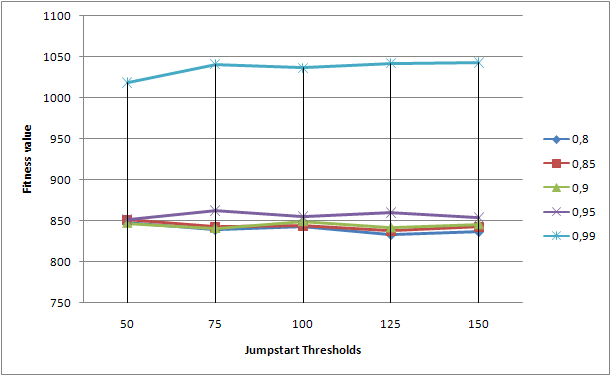
\includegraphics[width=\doubleimwidth]{tuning_jumpstart-vs-alpha.png}
  \label{fig:jumpstart-vs-alpha}
}

\subfloat[Starting temperatures versus jumpstart threshold values]{
  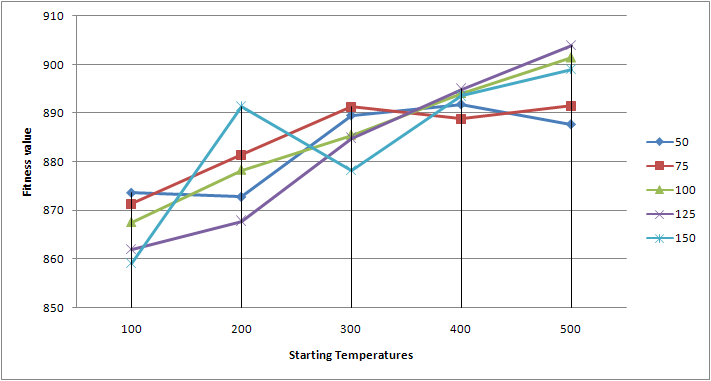
\includegraphics[width=\doubleimwidth]{tuning_starttemp-vs-jumpstart.png}
  \label{fig:starttemp-vs-jumpstart}
}

\subfloat[Starting temperatures versus cooling factors]{
  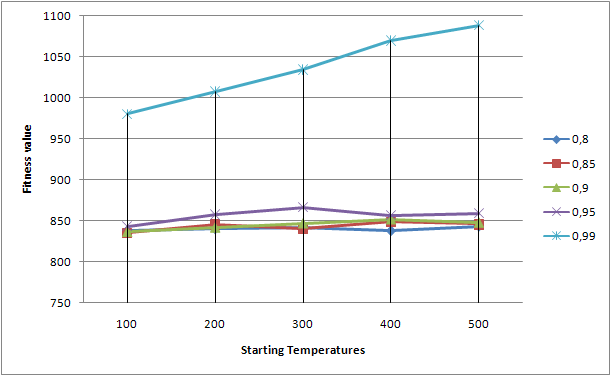
\includegraphics[width=\doubleimwidth]{tuning_starttemp-vs-alpha.png}
  \label{fig:starttemp-vs-alpha}
}
\caption{Effects of parameter variations}
\end{figure}

In Figures (\ref{fig:jumpstart-vs-alpha}-\ref{fig:starttemp-vs-alpha}) are the average fitness values of all 2-combinations of parameters where lower is better. Each parameter combination was tested 10 times and the fitness is the average of the final solution values. 

The running time of the solver was $0.1$ seconds since convergence was quickly achieved in the small networks available - Herlev and Glostrup. It was observed that in at most 1 second simulated annealing with any parameter combination would have found almost identical solutions, indicating that an optimum solution has been found under the chosen evaluation scheme.

The parameter, which is most sensitive, seems to be alpha, which must not be too high. In Figures \ref{fig:starttemp-vs-alpha} and \ref{fig:jumpstart-vs-alpha} we see that alpha = $0.99$ gives considerably worse fitness values and taking alpha down to $0.95$ reduces the gap in fitness. The best alpha value is $0.9$ by a minor margin indicating that the best solutions are found by - relatively quickly - decreasing the capability of accepting a worse-than-current solution.

The jumpstart threshold value is not very sensitive, which is seen in Figures \ref{fig:jumpstart-vs-alpha} and \ref{fig:starttemp-vs-jumpstart} in that it is mainly the variation in the other parameter (cooling factor and starting temperature resp.) that causes changes of fitness. We can deduce from this that the jumpstart actions are not of high importance to simulated annealing in this problem.

The best starting temperature among the tested values is 100 again supporting the claim that the solver desires to quickly zoom in on a specific region of the search space. Using this temperature and the best alpha value of $0.90$, we see in Figure \ref{fig:cooling_scheme} the resulting cooling.

\begin{figure}[htbp]
\centering
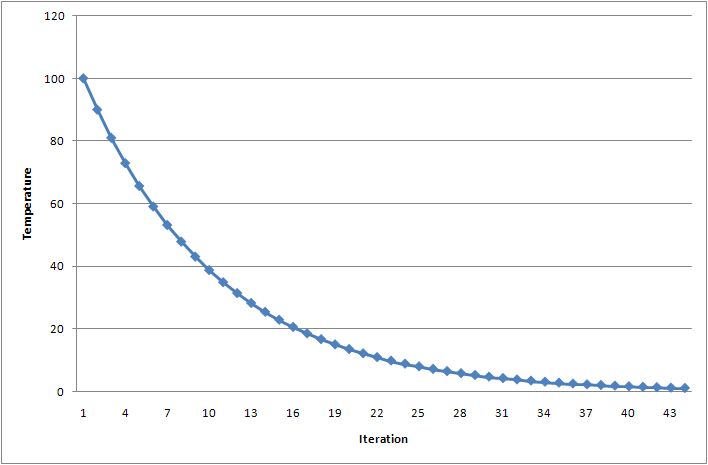
\includegraphics[width=0.5\textwidth]{temp-vs-iter_alpha09_starttemp100.png}
\caption{Cooling diagram for alpha $0.9$ and starting temperature $100$.}
\label{fig:cooling_scheme}
\end{figure}

The final results of the parameter tuning, which was used in the final testing, can be seen in Table \ref{tab:saparms}.

\begin{table}[htbp]
\centering
\begin{tabular}{l|c}
\textbf{Parameter} & \textbf{Value}\\ \hline
Starting temperature & 100 \\
Cooling factor (alpha) & 0.9 \\ 
Jumpstart threshold & 75 \\
Reheat action probability & 0.33 \\
Focus action probability & 0.33 \\
Random restart action probability & 0.33 \\
Offset change probability & 1.0 \\
Speed change probability & 0.0
\end{tabular}
\caption{Parameters used for simulated annealing when generating offsets for the tests in section \ref{test}.}
\label{tab:saparms}
\end{table}

\subsubsection*{Effect of speed changes on fitness values}
A neighbor solution is different by the speed in a coordination \textit{or} by an offset and thus when creating the neighbor solution it must be decided which change to make.
Maintaining the values of Table \ref{tab:saparms} except for speed and offset change probabilities I have performed another test to see the effect of making speed changes compared to changing offsets.

\begin{figure}[htbp]
\centering
\subfloat[All probabilities]{
  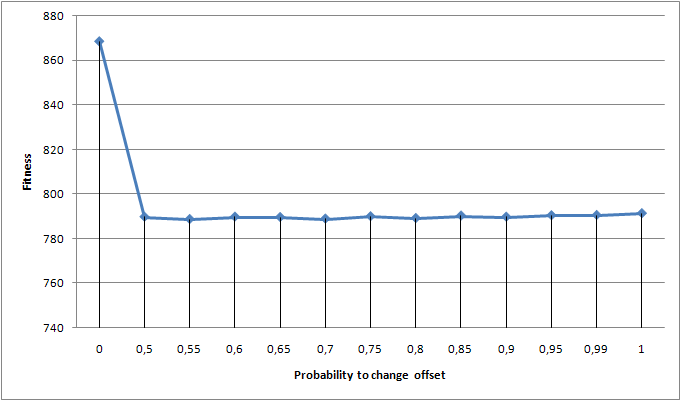
\includegraphics[width=\doubleimwidth]{tuning_change_offset-speed_ratio0.png}
  \label{fig:offset-vs-speed0}
}
\subfloat[All probabilities but zero]{
  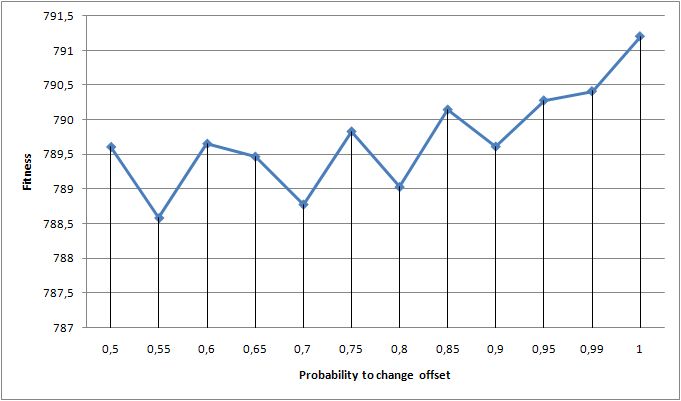
\includegraphics[width=\doubleimwidth]{tuning_change_offset-speed_ratio.png}
  \label{fig:offset-vs-speed}
}
\caption{Probability of changing offsets and speeds}
\end{figure}

In Figure \ref{fig:offset-vs-speed0} we see the importance of offsets compared to the average speeds used between intersections. In Figure \ref{fig:offset-vs-speed} we are zoomed in on the upper probability levels for changing offsets and see that, although marginal, allowing speed changes with probability $0.3$ is preferable to not allowing speed changes at all.